\section{Задание 2}
    \begin{enumerate}
        \item Построить датчик сингулярного распределения, имеющий в качестве 
        функции распределения канторову лесницу. С помощью критерия Колмогорова 
        убедиться в корректности работы датчика.
        \item Для канторовых случайных величин проверить свойство симметричности 
        относительно $\frac{1}{2}$ ($X$ и $1 - X$ распределены одинаково) и 
        самоподобия относительно деления на 3 (условное распределение $Y$ при 
        условии $Y \in \segm{0}{\frac{1}{3}}$ совпадает с распределением 
        $Y/3$) с помощью критерия Смирнова.
        \item Вычислить значение математического ожидания и дисперсии для 
        данного распределения. Сравнить теоретические значения с эмпирическими 
        для разного объема выборок. Проиллюстрировать сходимость.
    \end{enumerate}

    \subsection{Датчик для канторова распределения}
        Случайная величина имеет канторово распеделение, если ее функция 
        распределения~--- канторова лестница.

        Носителем канторова распределения является канторово множество, 
        представимое как счетное пересечение множеств

        \begin{align*}
            C_0 = {} & [0,1] \\
            C_1 = {} & [0,1/3] \cup [2/3,1] \\
            C_2 = {} & [0,1/9] \cup [2/9,1/3] \cup [2/3,7/9] \cup [8/9,1] \\
            \cdots, & \\
            C_n = & \bigcup_{i = 1,\ldots, 2^n}{\segm{a_i}{b_i}}
        \end{align*}

        Причем $\Prb{\segm{a_i}{b_i}} = \dfrac{1}{2^n},\:\forall i$, что дает 
        естественный способ разложения сл.в. $\delta~\sim~\mathrm{Cant}$ в ряд 
        по  $\xi~\sim~\mathrm{Bern(0.5)}$

        \begin{equation}\label{cauchy_series}
            \delta = \sum\limits_{i = 1}^{\infty} \dfrac{2}{3^i}\xi_i.
        \end{equation}

        Таким образом, для моделирования канторовской случайной величины 
        достаточно провести достаточно большое число испытаний бернулли и 
        посчитать сумму приближающую ряд \eqref{cauchy_series}.

        \begin{figure}[tbp]
            \centering
            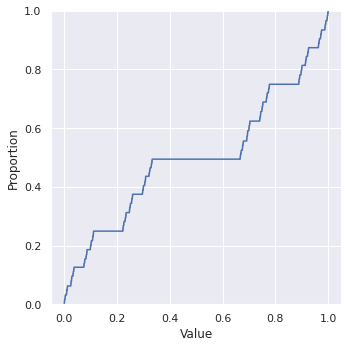
\includegraphics[width=0.5\textwidth]{resources/task2_cantor.png}
            \caption{Э.ф.р. канторовой сл.в.}
            \label{task1_cantor}
        \end{figure}
        
        \bigskip
        
        Для проверки корректности полученного датчика напомним следующee.

        Статистикой критерия Колмогорова является величина 
        \[\sqrt{n}D_n = \sup\limits_{-\infty < x < \infty} 
                                                \abs{\widehat F_n(x) - F(x)},\]
        где $\widehat F_n(x) = \dfrac{1}{n}\sum\limits_{i=1}^{n} 
        \Ind{X_i \le x}$~--- эмпирическая функция распределения.

        \begin{theorem}[Колмогоров] Если функция распределения элементов выборки 
            $F(x)$ непрерывна, то для $x > 0$
            \[\lim_{n\rightarrow\infty}\Prb{\sqrt{n}D_n \le x} = K(x) = 
            1 + 2\sum\limits_{k=1}^{\infty}(-1)^k e^{-2k^2 x^2}.\]
        \end{theorem}

        Проверяемая гипотеза c заданным \emph{уровнем значимости $\alpha$} 
        отвергается, если на полученной выборке $(X_1,\ldots,X_n)$ значение 
        статистики неправдоподобно велико, т.е.
        \begin{equation}\label{rej_cond}
            \sqrt{n}D_n(X_1,\ldots,X_n) \ge x_{1-\alpha},
        \end{equation}
        где $x_{1-\alpha}$~--- наименьшее значение, удовлетворяющее условию
        \[\Prb{\sqrt{n}D_n \ge x_{1-\alpha}} \le \alpha.\]

        В силу теоремы Колмогорова ``в пределе'' 
        \[\Prb{\sqrt{n}D_n \ge x_{1-\alpha}} = 1 - K(x_{1-\alpha}) = 
                                                    1 - (1-\alpha) = \alpha,\]
        и $\: x_{1-\alpha}$ есть не что иное как $(1-\alpha)$-квантиль функции 
        $K(x)$.                                                    

        Таким образом для значения статистики $\sqrt{n}D_n(X)$ на некоторой 
        определенной выборке $X$ справедливо

        \[\Prb{\sqrt{n}D_n \ge \sqrt{n}D_n(X)} = 1 - K(\sqrt{n}D_n(X)) = 
        1 - (1-\alpha(X)) = \alpha(X)\]

        тем самым $\sqrt{n}D_n$~--- $(1-\alpha(X))$-квантиль, и условие 
        \eqref{rej_cond} выполнено для тех и только тех $x_{1-\alpha}$, что 
        \begin{gather*}
            x_{1-\alpha(X)} \ge x_{1-\alpha} \Leftrightarrow \\
            1-\alpha(X) \ge 1-\alpha \Leftrightarrow \\
            \alpha \ge \alpha(x)
        \end{gather*}

        Выходит что для полученной в результате серии испытаний статистики 
        $\sqrt{n}D_n(X)$ значение $1 - K(\sqrt{n}D_n(X)) = \alpha(X)$ означает, 
        что гипотезу \emph{следует отвергнуть} тогда и только тогда, когда был 
        принят уровень значимости $\alpha$ больший чем величина $\alpha(X)$. И 
        обратно, гипотеза \emph{может быть принята} для любого уровня значимости 
        $\alpha$ меньшего чем $\alpha(X).$
        
        Поскольку функция $F(x)$ непрерывна и не убывает, а $\hat F_n(x)$~--- 
        кусочно-постоянна, то $D_n$ можно вычислить по формуле
        
        \[D_n(x_1,\ldots,x_n) = \max\limits_{1\le i \le n}
        \left\{\dfrac{1}{n} - F(x_{(i)}),\: F(x_{(i)}) - \dfrac{i-1}{n}\right\}.\]

        Посчитанная таким образом на некотрой выборке $(X_1,\ldots,X_n)$ 
        значений датчика $\delta$ статистика $D_n$ составляет приблизительно 
        $0.0087$. Величина $1-K(\sqrt{n}D_n) = \alpha(X)$ равна приблизительно 
        $0.9999$, что даёт нам основания принять гипотезу о корректности 
        построенного датчика $\delta$, с уровнем значимоcти, например, 20\%.

    \subsection{Свойства симметричности и самоподобия}
        Для проверки требуемых свойств необходимо к двум сгенерированным 
        выборкам $(X_1,\ldots,X_n),\; (Y_1,\ldots,Y_m)$ применить критерий 
        Смирнова, статистикой которого служит величина 
        \begin{gather*}
            D_{n,m} = \sup\limits_{x}\abs{\widehat F_n(x) - \widehat G_n(x)},\\
            \text{где } \widehat F_n(x) = \dfrac{1}{n}\sum\limits_{i=1}^{n} \Ind{X_i \le x},\quad
                        \widehat G_n(x) = \dfrac{1}{m}\sum\limits_{j=1}^{m} \Ind{Y_i \le x}.
        \end{gather*}

        Известен следующий результат
        \begin{theorem}[Смирнов] Если гипотеза однородонсти верна (подробнее см. 
            \cite{NMS}), то имеет место сходимость
            \[\Prb{\sqrt{nm/(n+m)} D_{n,m} \le x} \rightarrow K(x) 
                                            \text{ при } n,m \rightarrow \infty,\]  
            где $K(x)$~--- функция распределения Колмогорова.
        \end{theorem}

        Для нахождения статистики достаточно произвести вычисления по формулам
        \begin{gather*}
            D_{n,m} = \max\{D_{n,m}^+,D_{n,m}^-\},\\
            \text{где}\\
            D_{n,m}^+ = \sup\limits_{x} \left( \widehat F_n(x) - \widehat G_n(x) \right)
            = \max\limits_{1 \le i \le n} \left\{ \dfrac{i}{n} - \widehat G_n(X_{(i)}) \right\}\\
            D_{n,m}^- = \sup\limits_{x} \left( \widehat G_n(x) - \widehat F_n(x) \right)
            = \max\limits_{1 \le j \le m} \left\{ \dfrac{j}{m} - \widehat F_n(Y_{(j)}) \right\}. 
        \end{gather*}

        В результате компьютерных вычислений для случайных величин 
        $\delta$ и $1 - \delta$ получены значения $D_{n,m} \approx 0.489$ 
        и $1 - K(\sqrt{nm/(n+m)} D_{n,m}) \approx 0.1811$, что позволяет принять
        гипотезу об одиноковой распределенности на уровне значимости 10\%.

        Соответствующие результаты для $\delta/3$ и $\delta\bigr|_{\segm{0}{3}}$
        составляют приблизительно $0.3482$ и $0.1427$ соответственно, что 
        подтверждает свойство самоподобия на уровне значимости 10\%.

    \subsection{Математическое ожидание и дисперсия}
        Случайная величина $\delta$ обладает свойством самоподобия, т.е. для ее 
        функции распределения $F(\cdot)$ выполнено: 
        \begin{itemize}
            \item $F(x) = \dfrac{F(3x)}{2},\; \text{при } \dfrac{2}{3} < x < 1,$
            \item $F(x) = \dfrac{1}{2} + \dfrac{F(3x-2)}{2},\; \text{при } \dfrac{2}{3} < x < 1.$
        \end{itemize}
        Используя это свойство вычислим математическое ожидание
        \begin{multline*}
        \Exp{\delta} = \int\limits_{-\infty}^{+\infty} x \,dF(x) = 
            \int\limits_{0}^{1/3} x \,dF(x) + \int\limits_{2/3}^{1} x \,dF(x) =
            \dfrac{1}{2}\int\limits_{0}^{1/3} x \,dF(3x) + \\
        + \dfrac{1}{2}\int\limits_{2/3}^{1} x \,d(1/2+F(3x-2)) = 
            \dfrac{1}{2}\int\limits_{0}^{1} \dfrac{y}{3} \,dF(y) + 
            \dfrac{1}{2}\int\limits_{0}^{1} \dfrac{y+2}{3} \,dF(y) = \\
        \dfrac{1}{6}\int\limits_{0}^{1} y \,dF(y) + 
            \dfrac{1}{6}\int\limits_{0}^{1} y \,dF(y) + 
            \dfrac{1}{3}\int\limits_{0}^{1} \,dF(y) = 
        \dfrac{1}{3}\Exp{\delta} + \dfrac{1}{3}.
        \end{multline*}
        Следовательно 
        \[ \Exp{\delta} = \frac{1}{2}. \]

        Аналогично дисперсия:
        \begin{multline*}
        \Exp{\delta^2} = \int\limits_{0}^{1/3} x^2 \,dF(x) + 
            \int\limits_{2/3}^{1} x^2 \,dF(x) = 
                \dfrac{1}{2}\int\limits_{0}^{1} \left(\dfrac{y}{3}\right)^2 \,dF(y) + \\
            + \dfrac{1}{2}\int\limits_{0}^{1} \left(\dfrac{y+2}{3}\right)^2 \,dF(y) = 
                \dfrac{1}{9}\Exp{\delta^2} + \dfrac{2}{9}\Exp{\delta} + \dfrac{2}{9} = 
                \dfrac{1}{9}\Exp{\delta^2} + \dfrac{1}{3}.
        \end{multline*}
        Т.е.
        \[\Exp{\delta^2} = \dfrac{3}{8},\]
        и
        \[\Disp{\delta} = \Exp{(\delta - \Exp{\delta})^2} = 
        \Exp{\delta^2} - (\Exp{\delta})^2 = \dfrac{3}{8} - \dfrac{1}{4} = \frac{1}{8}\]
        
        Сходимость эмпирических показателей к теоретическим показана на рис. 
        \ref{task2_meanvar}.

        \begin{figure}[tbp]
            \centering
            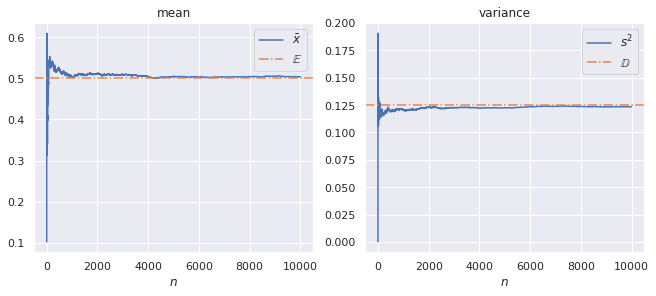
\includegraphics[width=1.0\textwidth]{resources/task2_meanvar.png}
            \caption{}
            \label{task2_meanvar}
        \end{figure}